%!TEX root = ../../thesis.tex

The first theory of weak interactions was a four-point interaction with coupling parameter 
$G_F$ = \unit{$1.166\times 10^{-5}$}{\GeV\rpsquared}, the Fermi constant. Although 
remarkably successful in describing low energy phenomena, such as nuclear $\beta$-decay, 
the theory experiences serious issues at high energies - predicting cross sections which 
scale with \ac{CM} energy $E$ like $\sigma \sim G_F^2 E^2$. These violate unitarity at 
$E \gtrsim \unit{300}{\GeV}$ \cite{Aitchison}.

The solution was to mediate the weak interaction through the exchange of electrically 
charged vector bosons (known as \PWpm bosons), similar to the exchange of photons in 
\ac{QED}. However, unlike \ac{QED}, the weak interaction is short ranged and therefore 
its exchange bosons must be massive. Since the propagator for a particle of mass $m$ and 
momentum $p$ contains $1 / (p^2 - m^2)$, in the low energy limit we identify that
\begin{equation}
	G_F \sim g^2 / m_{\PW}^2 ,
\end{equation}
where $g$ is the coupling of the vector boson. Thus, at low energies, the strength of the weak interaction is suppressed by the mass of the exchange boson.

At this time, there were two key obstacles to unifying the electromagnetic and weak 
interactions into a single interaction. Firstly, following the experimental discovery of 
parity violation in the $\beta$-decay of cobalt-60 \cite{Wu:1957}, the weak interaction
was known to have a \VminusA structure whereas \ac{QED} has a pure V structure. 
Secondly, the weak interaction has massive gauge bosons whilst the photons of \ac{QED} are 
massless. This was a major problem because gauge bosons are inherently massless.\footnote{
	Consider the local gauge transformation of a Yang-Mills gauge field 
	$\bvec{W}^{\mu} \rightarrow \bvec{W}^{\mu} - \partial^{\mu} \bvec{\epsilon}(x)
	- g \lbrack \bvec{\epsilon}(x) \times \bvec{W}^{\mu} \rbrack$. Clearly the mass term 
	$-\tfrac{1}{2}m^2 \bvec{W}_{\mu} \cdot \bvec{W}^{\mu}$ is not gauge invariant, and 
	hence the gauge boson is massless.}
In fact, the chiral nature of the weak interaction forbids fermion masses too, which are
also experimentally observed.\footnote{
	Consider a spinor as the sum of its left- and right-handed chiral states 
	$\psi = \psi_L + \psi_R$. Then the Dirac mass term is $-m \bar{\psi} \psi = 
	-m (\bar{\psi}_R \psi_L + \bar{\psi}_L \psi_R)$. For a chiral theory, $\psi_L$ and
	$\psi_R$ behave differently under local gauge transformation and thus the mass term is not gauge invariant.
}

A major step was taken by Glashow in the proposal of an \EWgroup group 
\cite{Glashow:1961}. This model describes three gauge fields 
\rowthreevec{W^1_{\mu}}{W^2_{\mu}}{W^3_{\mu}} which couple to weak isospin $T$ with 
strength $g$, and a single gauge field $B_{\mu}$ which couples to weak hypercharge $Y$ 
with strength $g'$. The subscript `$L$' indicates that only left-handed chiral particles 
couple to the $W^i_{\mu}$ fields, explaining the \VminusA nature of the weak interaction. 
The physical gauge fields are obtained through the mixing of these fields, with weak mixing
angle $\theta_W$:
\begin{align}
	W^{\pm}_{\mu} &= (W^1_{\mu} \mp i W^2_{\mu}) / \sqrt{2} \\
	A_{\mu} &= \sin\theta_W W^3_{\mu} + \cos\theta_W B_{\mu} \\
	Z_{\mu} &= \cos\theta_W W^3_{\mu} - \sin\theta_W B_{\mu} ,
\end{align}
where $W^{\pm}_{\mu}$ leads to the electrically charged \PWpm bosons, $A_{\mu}$ leads to
the photon and $Z_{\mu}$ leads to a new neutral \PZ boson. Weak neutral currents were a 
prediction of the theory and were later confirmed experimentally. 
\todo[inline]{Cite Gargamelle neutrino experiment?}

Glashow's \EWgroup theory therefore predicts the interaction of fermions, in left-handed 
\SUgroup{2} doublets and right-handed \SUgroup{2} singlets, with \PWpm, \PZ and \Pphoton 
exchange bosons. Gauge boson self-interactions are also expected due to the non-abelian 
nature of the \ac{EW} theory. The \PWpm bosons couple to weak isospin $T$ with strength 
$g$, the \PZ boson couples vectorially to $c_V$ and axially to $c_A$ with strength 
$g/(2\cos\theta_W)$, and the photon couples to electric charge $Q$ with strength 
$e = g\sin\theta_W$, where
\begin{align}
	c_V &= T_3 - 2 Q \sin^2\theta_W & c_A &= T_3 \\
	Q   &= T_3 + \frac{Y}{2}
\end{align}
and $T_3$ is the third component of weak isospin. The relevant quantum numbers of each
fermion are displayed in \Table~\ref{tab:ew_fermions}.

\begin{table}
	\begin{tabular}{ccc@{\hskip 1cm}cccc}
		& & & $T$ & $T_3$ & $Y$ & $Q$ \\
		\hline
		\multirow{2}{*}{$\colvector{\Pnue\\ \Pe}_{\!\!\!L}$} & 
		\multirow{2}{*}{$\colvector{\Pnum\\ \Pmu}_{\!\!\!L}$} & 
		\multirow{2}{*}{$\colvector{\Pnut\\ \Ptau}_{\!\!\!L}$} & 
		$\tfrac{1}{2}$ & $+\tfrac{1}{2}$ & $-1$ & 0 \\
		& & & $\tfrac{1}{2}$ & $-\tfrac{1}{2}$ & $-1$ & $-1$ \\
		$\Pnue_R$ & $\Pnum_R$ & $\Pnut_R$ & 0 & 0 & 0 & 0 \\
		$\Pe_R$ & $\Pmu_R$ & $\Ptau_R$ & 0 & 0 & $-2$ & $-1$ \\
		\hline
		\multirow{2}{*}{$\colvector{\Pup\\ \Pdown'}_{\!\!\!L}$} & 
		\multirow{2}{*}{$\colvector{\Pcharm\\ \Pstrange'}_{\!\!\!L}$} & 
		\multirow{2}{*}{$\colvector{\Ptop\\ \Pbottom'}_{\!\!\!L}$} & 
		$\tfrac{1}{2}$ & $+\tfrac{1}{2}$ & $+\tfrac{1}{3}$ & $+\tfrac{2}{3}$ \\
		& & & $\tfrac{1}{2}$ & $-\tfrac{1}{2}$ & $+\tfrac{1}{3}$ & $-\tfrac{1}{3}$ \\
		$\Pup_R$ & $\Pcharm_R$ & $\Ptop_R$ & 0 & 0 & $+\tfrac{4}{3}$ & $+\tfrac{2}{3}$ \\
		$\Pdown'_R$ & $\Pstrange'_R$ & $\Pbottom'_R$ & 0 & 0 & $-\tfrac{2}{3}$ & $-\tfrac{1}{3}$ \\
	\end{tabular}
	\caption{The weak isospin $T$, weak hypercharge $Y$ and electric charge $Q$ quantum
	numbers assigned to the fermions. Right-handed neutrinos are decoupled from the 
	electroweak interaction, and were not originally included in the \ac{SM}. However, 
	recent observations of neutrino oscillations suggest that these might in fact exist.}
	\label{tab:ew_fermions}
\end{table}

Unfortunately, it was necessary to manually break the \ac{EW} symmetry to give masses to 
the \PWpm and \PZ bosons. Initial attempts to invoke a mechanism of spontaneous symmetry 
breaking were hindered by the Goldstone Theorem.



\subsection{The Goldstone Theorem}
\label{sec:ewsb:goldstone}
Sombrero
Difficulties in breaking electroweak symmetry due to Goldstone theorem predicting massless scalar Nambu-Goldstone bosons (not experimentally observed)

\begin{figure}
	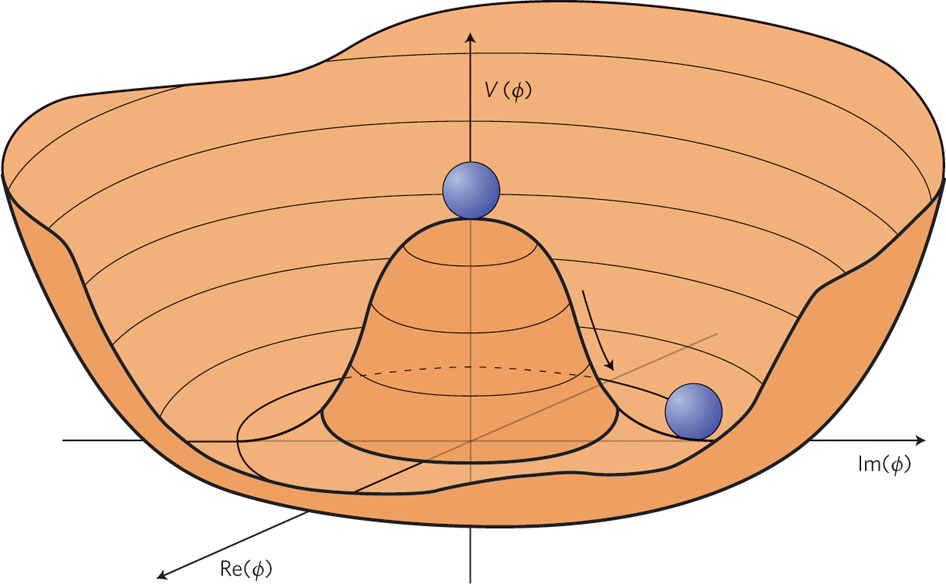
\includegraphics[width=\mediumfigwidth]{tex/motivation/sombrero}
	\caption{The sombrero potential, in which a vacuum state must be arbitrarily chosen, 
	spontaneously breaking the symmetry of the underlying Lagrangian.
	Fluctuations in the azimuthal direction correspond to a massless Nambu-Goldstone 
	boson. Fluctuations in the radial direction correspond to a massive Higgs boson.}
	\label{fig:sombrero}
\end{figure}

\subsection{The Higgs Mechanism}
\label{sec:ewsb:higgs}
Abelian Higgs model
Superconductivity done by Anderson for non-relativistic theory (Meissner effect since photons eat Goldstone bosons, massive mode in Raman spectrum is Higgs boson)
Apply Higgs mechanism to non-abelian theories (Kibble)
Weinberg and Salam independently applied to EW
Gave relation between W and Z masses

\begin{equation*}
\SUgroup{2}_{L} \times \Ugroup{1}_{Y} \xrightarrow{\text{EWSB}} \Ugroup{1}_{Q}
\end{equation*}
